\documentclass{article}
\usepackage[utf8]{inputenc}
\usepackage{graphicx}
\usepackage[a4paper,width=150mm,left=5mm,right=5mm,top=5mm,bottom=15mm]{geometry}
\usepackage{booktabs}  % nice tables
\usepackage{placeins}  % \FloatBarrier to stop float drift
\usepackage{caption}   % consistent captions if needed

\title{
{
\includegraphics{../assets/usask.png}} \ {
\includegraphics[width=40mm]{../assets/uregina.png}}\\
{Acoustic Signal Classification}\\
{\large Final Report}\\
}

\author{Kanwar Pannu\\ Supervised by: Dr. Travis Wiens , Dr. Abdul Bais}

\begin{document}

\maketitle

\begin{abstract}
This report presents the findings of a project focused on classifying acoustic signals from mine roofs to assess their safety. The classification is based on audio recordings labeled as ``Drummy'' or ``Tight'', indicating the condition of the mine roof. The project utilized machine learning techniques to analyze and classify these audio signals, contributing to improved safety measures in mining operations. The results demonstrate the effectiveness of the developed models in accurately identifying roof conditions based on acoustic data.\\
\end{abstract}

\newpage
\section{Background and Project Overview}
Evaluating whether an impact sounds tight or drummy is a subjective skill that requires training and experience. Challenging conditions (e.g., intersecting rooms, high roofs) can make this judgment difficult even for experts. This project records the sound of scaling-bar impacts and uses machine learning to classify them as either ``Tight'' or ``Drummy'', reducing subjectivity.
\noindent\textbf{Phase 2 Device Functionality:}
\begin{itemize}
  \item Detect impacts and record audio.
  \item Optional in-field labeling (drummy/tight).
  \item Transmit audio via Bluetooth to the app.
  \item Receive classifier results and display via RGB LED.
\end{itemize}

\begin{figure}[h]
  \centering
  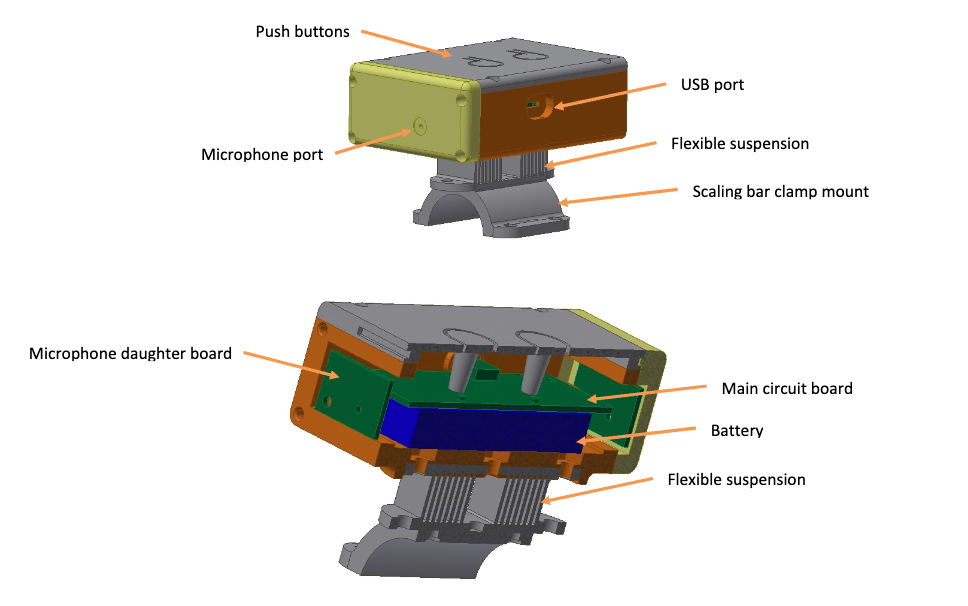
\includegraphics[width=50mm]{../assets/phase2_device.png}
  \caption{Phase 2 custom device mounted on a scaling bar.}
  \label{fig:phase2_device}
\end{figure}

\FloatBarrier

\newpage
\section{Understanding the Dataset}
\subsection{Phase 1}
Phase 1 consists of \textbf{3,309 recordings} (\textbf{2,212 drummy} and \textbf{1,097 tight}). Each recording is \textbf{0.75 s} long (\textbf{36{,}000 samples}) at \textbf{48 kHz}. The class distribution is imbalanced (drummy $\approx$ 2x tight), so any accuracy \(\le\) \textbf{66\%} is not better than a majority guess.

\begin{figure}[h]
    \centering
    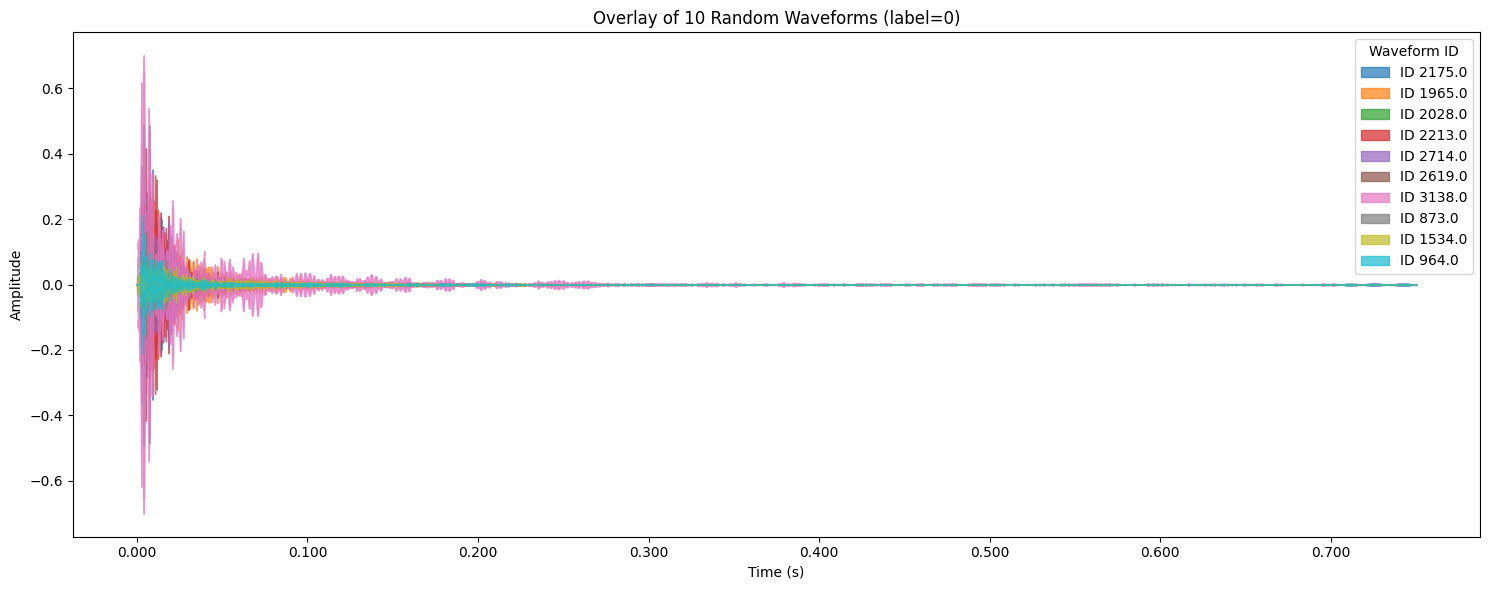
\includegraphics[width=0.8\textwidth]{../assets/final_report_assets/phase1_waveform_overlay_0.png}
    \caption{Waveform overlay of Phase 1 recordings — Label 0 (Drummy).}
    \label{fig:phase1_waveform_overlay_0}
\end{figure}
\begin{figure}[h]
    \centering
    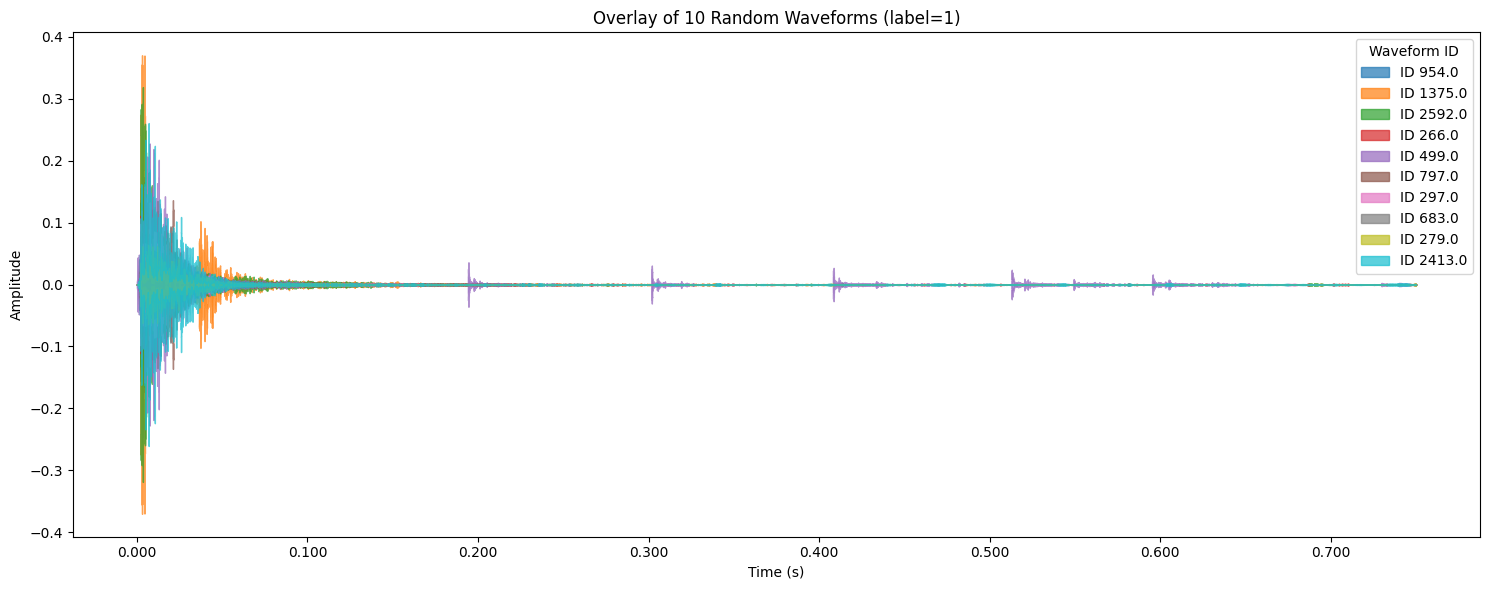
\includegraphics[width=0.8\textwidth]{../assets/final_report_assets/phase1_waveform_overlay_1.png}
    \caption{Waveform overlay of Phase 1 recordings — Label 1 (Tight).}
    \label{fig:phase1_waveform_overlay_1}
\end{figure}

\FloatBarrier
\newpage
\subsection{Phase 2}
Raw Phase 2 contains \textbf{9,923} recordings; \textbf{1,483} were \textbf{NaN-corrupted} ($\Rightarrow$ 8,440). In addition, \textbf{mishits} (non-impacts/invalid recordings) were identified and removed by waveform screening, yielding a final dataset of \textbf{8,229} recordings. Each has \textbf{4,800 samples} (\textbf{0.1 s} at \textbf{48 kHz}). Classes are more balanced; any accuracy \(\le\) \textbf{54\%} is not better than a majority guess.

\begin{figure}[h]
    \centering
    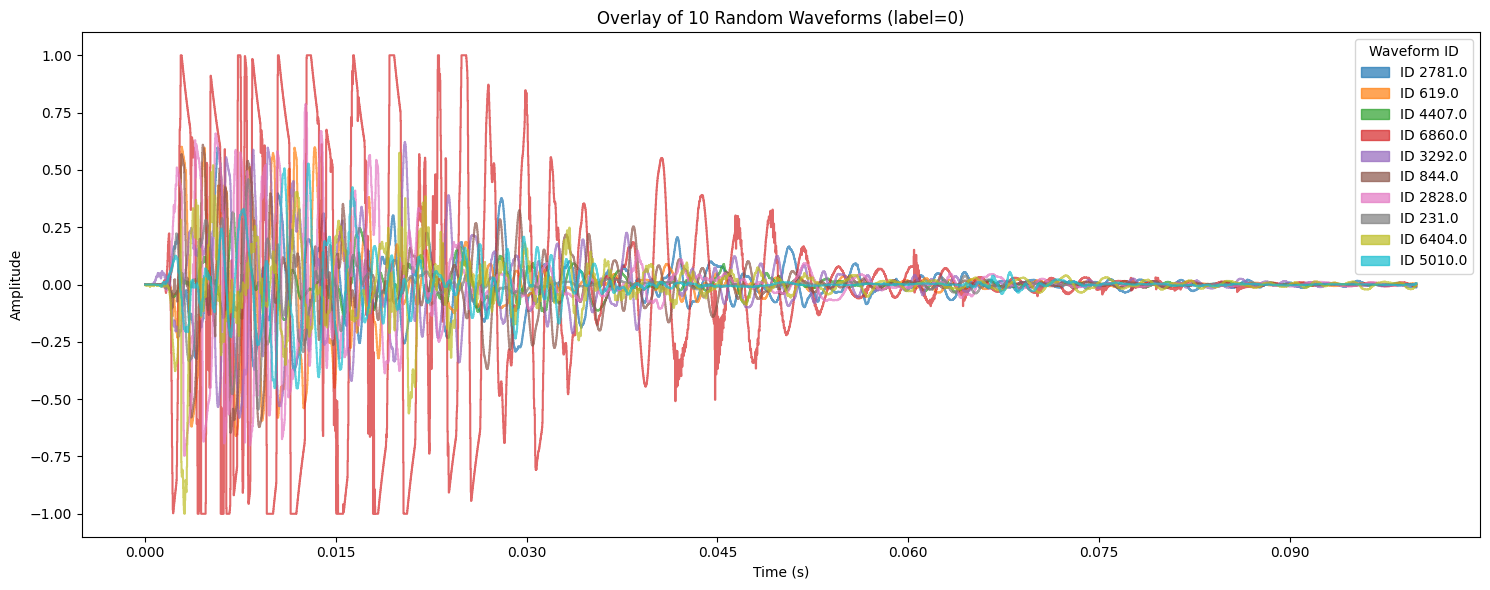
\includegraphics[width=0.8\textwidth]{../assets/final_report_assets/phase2_waveform_overlay_0.png}
    \caption{Waveform overlay of Phase 2 recordings — Label 0 (Drummy).}
    \label{fig:phase2_waveform_overlay_0}
\end{figure}
\begin{figure}[h]
    \centering
    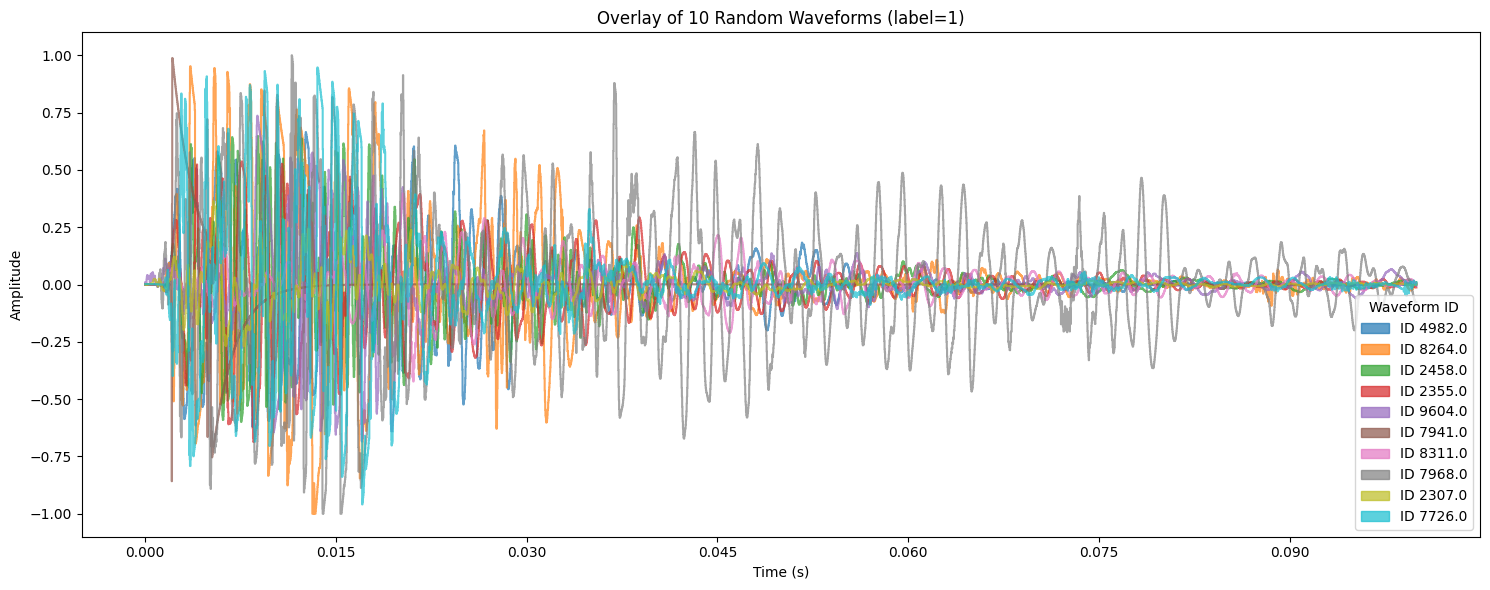
\includegraphics[width=0.8\textwidth]{../assets/final_report_assets/phase2_waveform_overlay_1.png}
    \caption{Waveform overlay of Phase 2 recordings — Label 1 (Tight).}
    \label{fig:phase2_waveform_overlay_1}
\end{figure}
\newpage
\subsection{Mishits}
Mishits were identified by visual inspection of the waveform and spectrogram.
\begin{figure}[h]
  \centering
  % 2x2 grid without subcaption
  \begin{minipage}{0.45\textwidth}\centering
    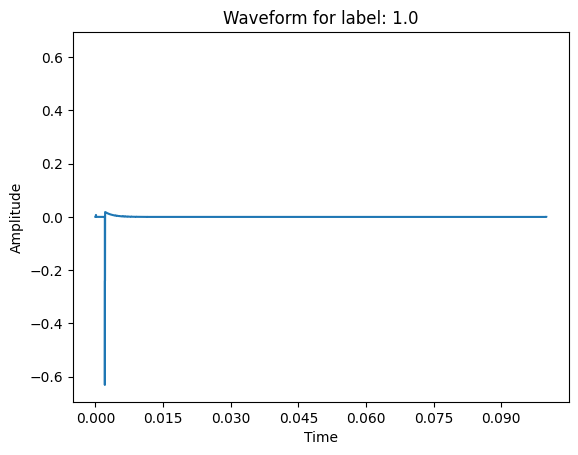
\includegraphics[width=0.95\linewidth]{../assets/phase2_mishit_1.png}
    \captionof{figure}{Phase 2 mishit (Tight).}
  \end{minipage}\hfill
  \begin{minipage}{0.45\textwidth}\centering
    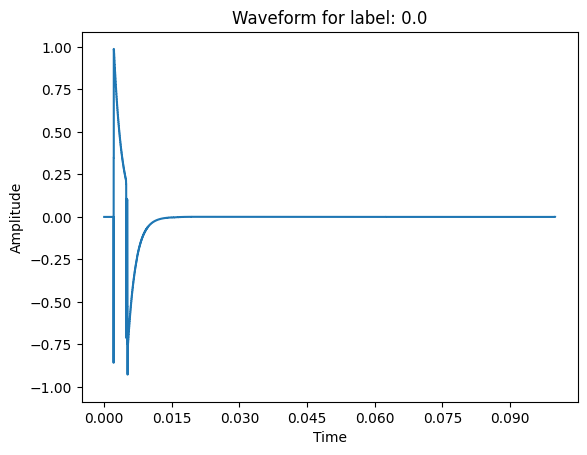
\includegraphics[width=0.95\linewidth]{../assets/phase2_mishit_0.png}
    \captionof{figure}{Phase 2 mishit (Drummy).}
  \end{minipage}

  \medskip

  \begin{minipage}{0.45\textwidth}\centering
    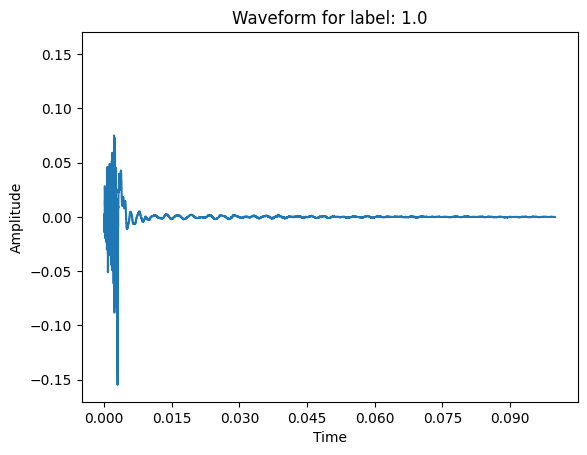
\includegraphics[width=0.95\linewidth]{../assets/phase2_mishit_1_1.png}
    \captionof{figure}{Phase 2 mishit (Tight).}
  \end{minipage}\hfill
  \begin{minipage}{0.45\textwidth}\centering
    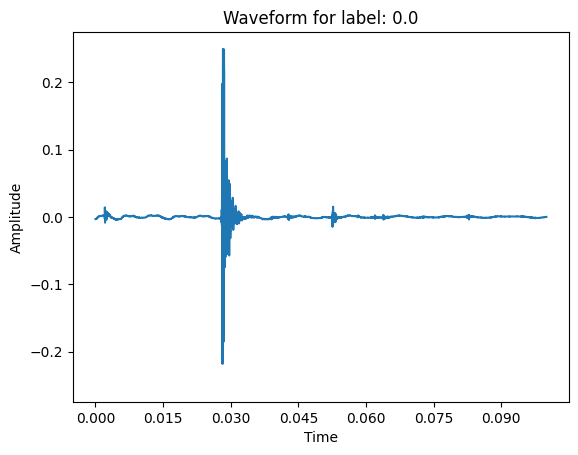
\includegraphics[width=0.95\linewidth]{../assets/phase2_mishit_0_1.png}
    \captionof{figure}{Phase 2 mishit (Drummy).}
  \end{minipage}
  \label{fig:phase2_mishits}
\end{figure}

\FloatBarrier

\newpage
\section{PCA as Feature Extraction}
PCA was used for dimensionality reduction; explained variance guided feature count. We compared SVM and MLP; \textbf{MLP consistently outperformed SVM}. Split: \textbf{80\% train / 20\% test}.

\subsection{Phase 1}
\begin{figure}[h]
    \centering
    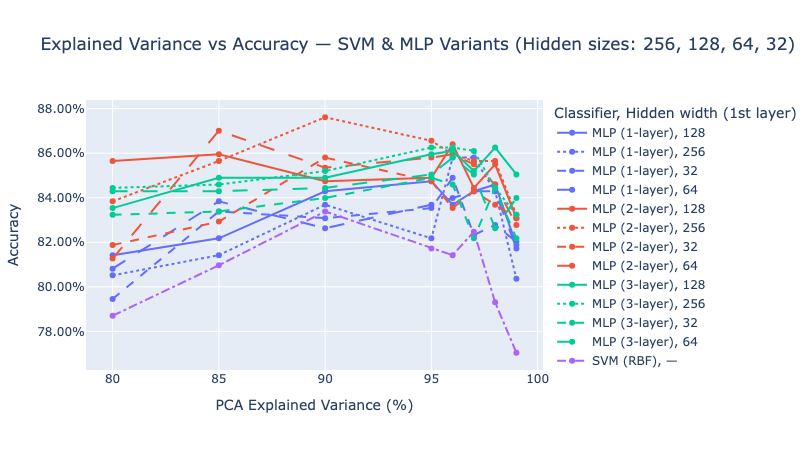
\includegraphics[width=0.8\textwidth]{../assets/final_report_assets/phase1_pca_explained_variance.png}
    \caption{Phase 1 — PCA explained variance vs model accuracy (multiple models).}
    \label{fig:phase1_pca_explained_variance}
\end{figure}

\noindent\textbf{Best Model and Feature Combination:}\\
\emph{90\% explained variance}, \emph{MLP with 2 hidden layers} (256, 128), \emph{dropout 0.2}.

\begin{table}[h]
\centering
\caption{Phase 1 PCA — Best model classification report.}
\begin{tabular}{@{}lccc r@{}}
\toprule
{} & precision & recall & f1-score & support \\
\midrule
drummy (0)   & 0.88 & 0.91 & 0.89 & 443 \\
tight (1)    & 0.80 & 0.74 & 0.77 & 219 \\
\midrule
accuracy     & \multicolumn{3}{c}{0.85} & 662 \\
macro avg    & 0.84 & 0.83 & 0.83 & 662 \\
weighted avg & 0.85 & 0.85 & 0.85 & 662 \\
\bottomrule
\end{tabular}
\end{table}

\begin{figure}
    \centering
    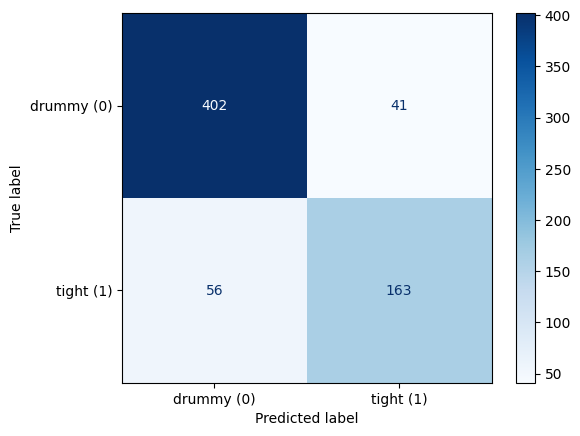
\includegraphics[width=0.3\textwidth]{../assets/final_report_assets/phase1_pca_best_confusion.png}
    \caption{Phase 1 PCA — Best model confusion matrix.}
    \label{fig:phase1_pca_best_confusion}
\end{figure}
\begin{figure}
    \centering
    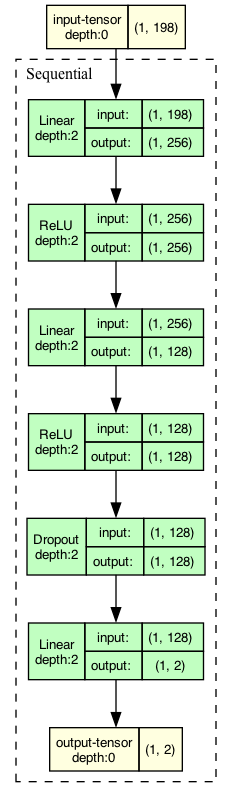
\includegraphics[width=0.4\textwidth]{../assets/final_report_assets/best_model_mlp2_ev90_h256_P1_RETRAIN.png}
    \caption{Phase 1 PCA — Best MLP architecture.}
    \label{fig:phase1_pca_best_model_architecture}
\end{figure}

\FloatBarrier
\newpage
\subsection{Phase 2}
\begin{figure}[h]
    \centering
    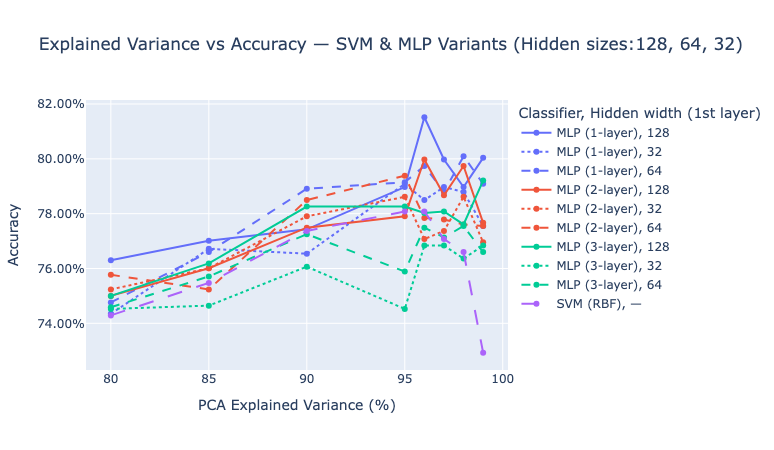
\includegraphics[width=0.8\textwidth]{../assets/final_report_assets/phase2_pca_explained_variance.png}
    \caption{Phase 2 — PCA explained variance vs model accuracy (multiple models).}
    \label{fig:phase2_pca_explained_variance}
\end{figure}

\noindent\textbf{Best Model and Feature Combination:}\\
\emph{96\% explained variance}, \emph{MLP with 1 hidden layer} (128), \emph{dropout 0.2}.

\begin{table}[h]
\centering
\caption{Phase 2 PCA — Best model classification report.}
\begin{tabular}{@{}lccc r@{}}
\toprule
{} & precision & recall & f1-score & support \\
\midrule
drummy (0)   & 0.78 & 0.86 & 0.82 & 926 \\
tight (1)    & 0.81 & 0.71 & 0.75 & 762 \\
\midrule
accuracy     & \multicolumn{3}{c}{0.79} & 1688 \\
macro avg    & 0.80 & 0.79 & 0.79 & 1688 \\
weighted avg & 0.79 & 0.79 & 0.79 & 1688 \\
\bottomrule
\end{tabular}
\end{table}

\begin{figure}[h]
    \centering
    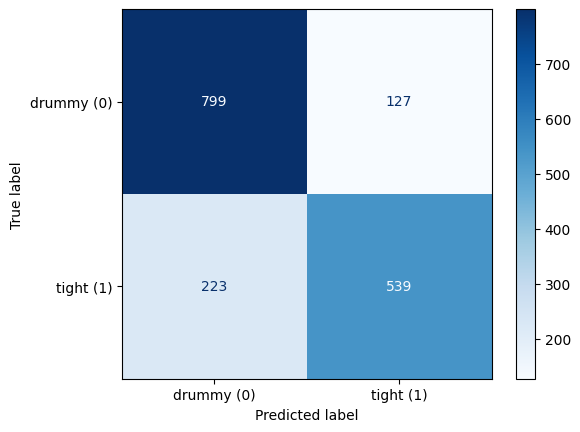
\includegraphics[width=0.3\textwidth]{../assets/final_report_assets/phase2_pca_best_confusion.png}
    \caption{Phase 2 PCA — Best model confusion matrix.}
    \label{fig:phase2_pca_best_confusion}
\end{figure}
\begin{figure}[h]
    \centering
    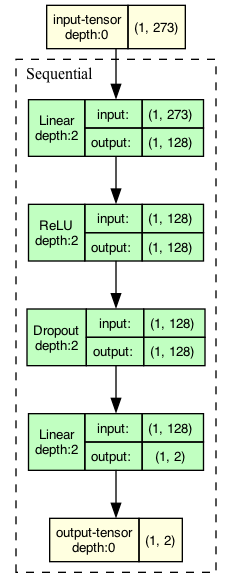
\includegraphics[width=0.4\textwidth]{../assets/final_report_assets/best_model_mlp1_ev96_h128_P2_RETRAIN.png}
    \caption{Phase 2 PCA — Best MLP architecture.}
    \label{fig:phase2_pca_best_model_architecture}
\end{figure}

\FloatBarrier
\newpage
\section{Deep Learning Models and Generalization Techniques}
PCA+MLP provided a strong baseline but cannot exploit the temporal structure of impacts. We therefore explored end-to-end CNNs and MFCC-based hybrids. Split: \textbf{90\% train / 10\% test}.

\noindent\textbf{Generalization:}
\begin{itemize}
  \item \textbf{Tanh} after convolutional stages: smoother feature maps and polarity preservation.
  \item \textbf{BatchNorm1d} on early residual outputs: stabilized feature statistics.
  \item \textbf{Dropout 0.6} in classifier heads: stronger regularization.
  \item \textbf{Label smoothing} $\epsilon=0.1$: mitigated overconfidence.
\end{itemize}

\newpage
\subsection{Phase 1 — ResNet (End-to-End)}
\noindent\textbf{Hyperparameters:} Epochs \(=20\), Batch size \(=32\), LR \(=10^{-3}\), Dropout \(=0.6\).

\begin{table}[h]
\centering
\caption{Phase 1 ResNet — Classification report.}
\begin{tabular}{@{}lccc r@{}}
\toprule
{} & precision & recall & f1-score & support \\
\midrule
drummy (0)   & 1.00 & 0.98 & 0.99 & 221 \\
tight (1)    & 0.96 & 0.99 & 0.97 & 88 \\
\midrule
accuracy     & \multicolumn{3}{c}{0.98} & 309 \\
macro avg    & 0.98 & 0.99 & 0.98 & 309 \\
weighted avg & 0.98 & 0.98 & 0.98 & 309 \\
\bottomrule
\end{tabular}
\end{table}

\begin{figure}[h]
  \centering
  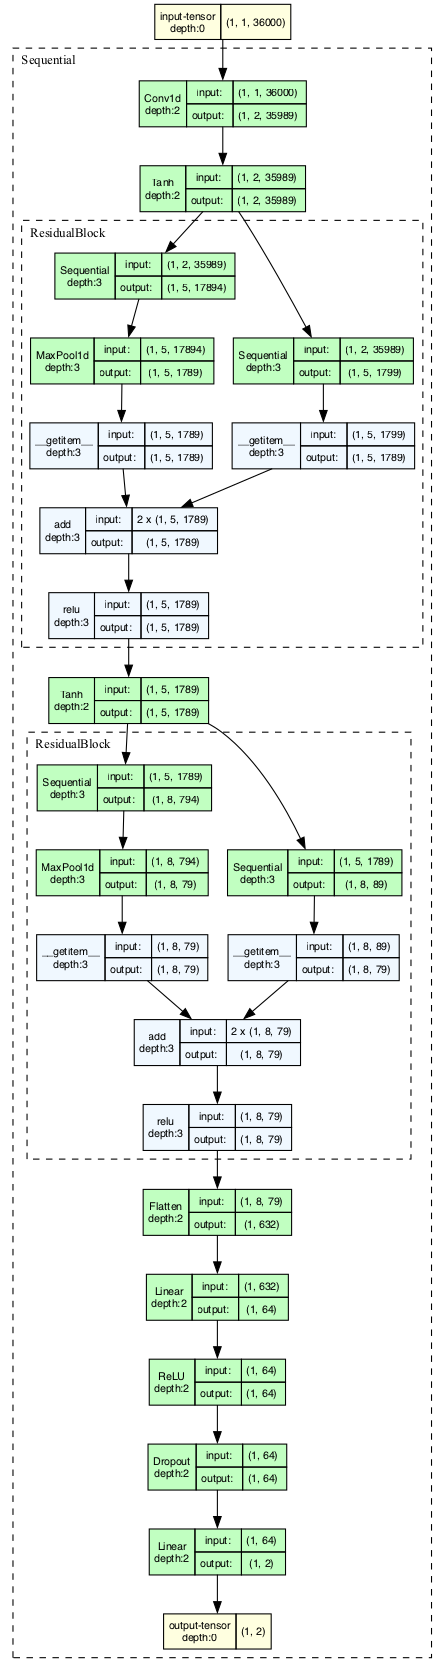
\includegraphics[width=0.15\textwidth]{../assets/final_report_assets/conv_p1_model_arch.png}
  \caption{Phase 1 CNN (ResNet-style) model architecture.}
  \label{fig:phase1_cnn_model_architecture}
\end{figure}
\begin{figure}[h]
  \centering
  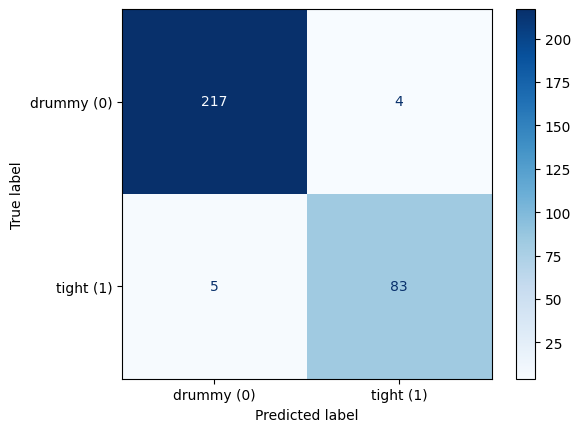
\includegraphics[width=30mm]{../assets/new_arch_conv_p1.png}
  \caption{Phase 1 ResNet — Confusion matrix.}
  \label{fig:phase1_resnet_confusion}
\end{figure}


\newpage
\subsection{Phase 2 — ResNet (End-to-End)}
\noindent\textbf{Hyperparameters:} Epochs \(=20\), Batch size \(=90\), LR \(=10^{-3}\), Dropout \(=0.6\), Weight decay \(=10^{-3}\).

\begin{table}[h]
\centering
\caption{Phase 2 ResNet — Classification report.}
\begin{tabular}{@{}lccc r@{}}
\toprule
{} & precision & recall & f1-score & support \\
\midrule
drummy (0)   & 0.87 & 0.92 & 0.90 & 466 \\
tight (1)    & 0.89 & 0.83 & 0.86 & 363 \\
\midrule
accuracy     & \multicolumn{3}{c}{0.88} & 829 \\
macro avg    & 0.88 & 0.88 & 0.88 & 829 \\
weighted avg & 0.88 & 0.88 & 0.88 & 829 \\
\bottomrule
\end{tabular}
\end{table}

\begin{figure}[h]
  \centering
  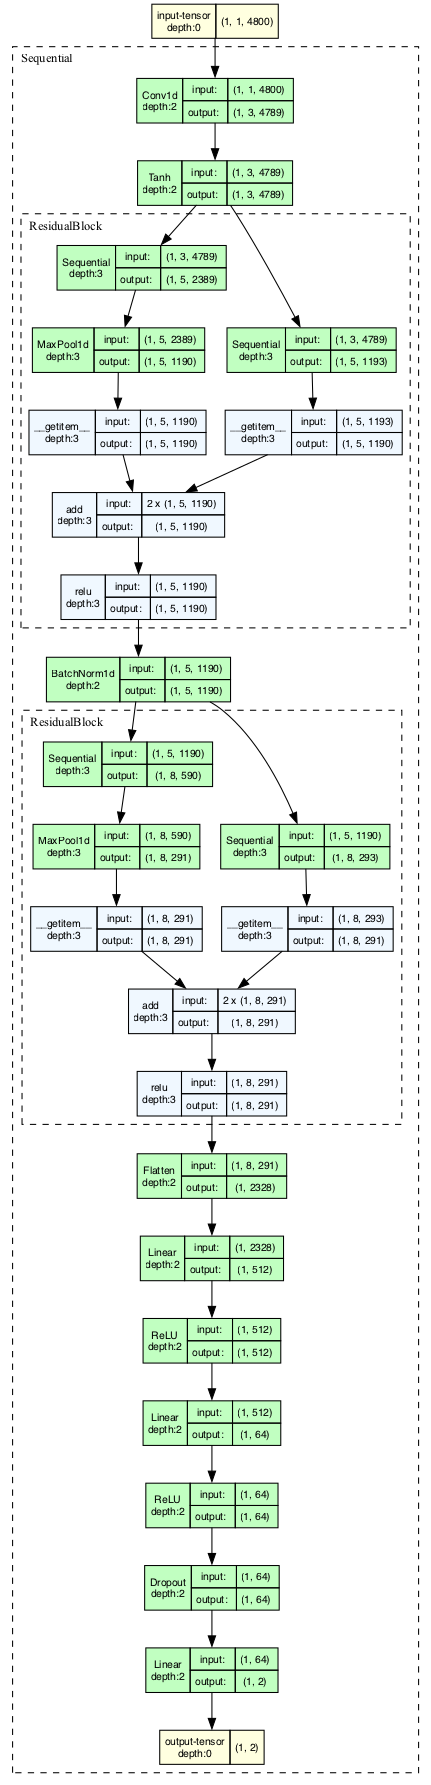
\includegraphics[width=0.15\textwidth]{../assets/final_report_assets/conv_p2_model_arch.png}
  \caption{Phase 2 CNN (ResNet-style) model architecture.}
  \label{fig:phase2_cnn_model_architecture}
\end{figure}
\begin{figure}[h]
  \centering
  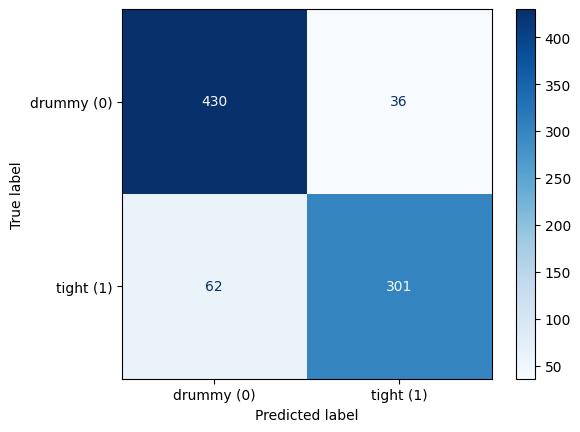
\includegraphics[width=25mm]{../assets/phase2_resnet_confusion.png}
  \caption{Phase 2 ResNet — Confusion matrix.}
  \label{fig:phase2_resnet_confusion}
\end{figure}

\newpage
\subsection{Phase 2 — MFCC + MLP}
\noindent\textbf{MFCC config:} \(n\_mfcc=40\), \(n\_fft=1024\), hop\_length \(=512\), \(n\_mels=40\). Input waveform shape \(\texttt{[1, 4800]}\).

\begin{table}[h]
\centering
\caption{Phase 2 MFCC + MLP — Classification report.}
\begin{tabular}{@{}lccc r@{}}
\toprule
{} & precision & recall & f1-score & support \\
\midrule
drummy (0)   & 0.91 & 0.90 & 0.91 & 466 \\
tight (1)    & 0.88 & 0.89 & 0.88 & 363 \\
\midrule
accuracy     & \multicolumn{3}{c}{0.90} & 829 \\
macro avg    & 0.89 & 0.90 & 0.89 & 829 \\
weighted avg & 0.90 & 0.90 & 0.90 & 829 \\
\bottomrule
\end{tabular}
\end{table}

\begin{figure}[h]
  \centering
  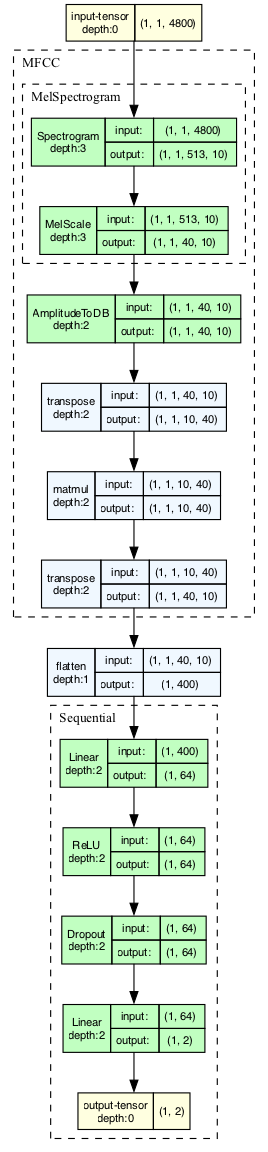
\includegraphics[width=0.15\textwidth]{../assets/final_report_assets/mfcc_p2_model_arch.png}
  \caption{Phase 2 MFCC + MLP — Model diagram.}
  \label{fig:phase2_MFCC_model_architecture}
\end{figure}
\begin{figure}[h]
  \centering
  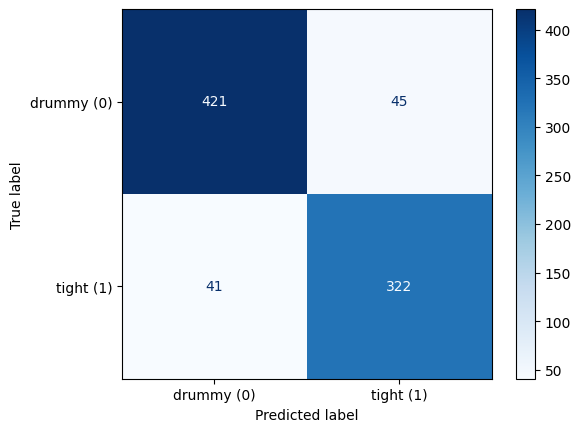
\includegraphics[width=20mm]{../assets/phase2_mfcc_mlp_confusion.png}
  \caption{Phase 2 MFCC + MLP — Confusion matrix.}
  \label{fig:phase2_mfcc_mlp_confusion}
\end{figure}

\newpage
\subsection{Phase 2 — MFCC + ResNet}
\noindent\textbf{Input:} MFCC feature maps; \textbf{Backbone:} ResNet-style CNN.

\begin{table}[h]
\centering
\caption{Phase 2 MFCC + ResNet — Classification report.}
\begin{tabular}{@{}lccc r@{}}
\toprule
{} & precision & recall & f1-score & support \\
\midrule
drummy (0)   & 0.94 & 0.93 & 0.93 & 466 \\
tight (1)    & 0.91 & 0.92 & 0.92 & 363 \\
\midrule
accuracy     & \multicolumn{3}{c}{0.93} & 829 \\
macro avg    & 0.92 & 0.93 & 0.93 & 829 \\
weighted avg & 0.93 & 0.93 & 0.93 & 829 \\
\bottomrule
\end{tabular}
\end{table}

\begin{figure}[h]
  \centering
  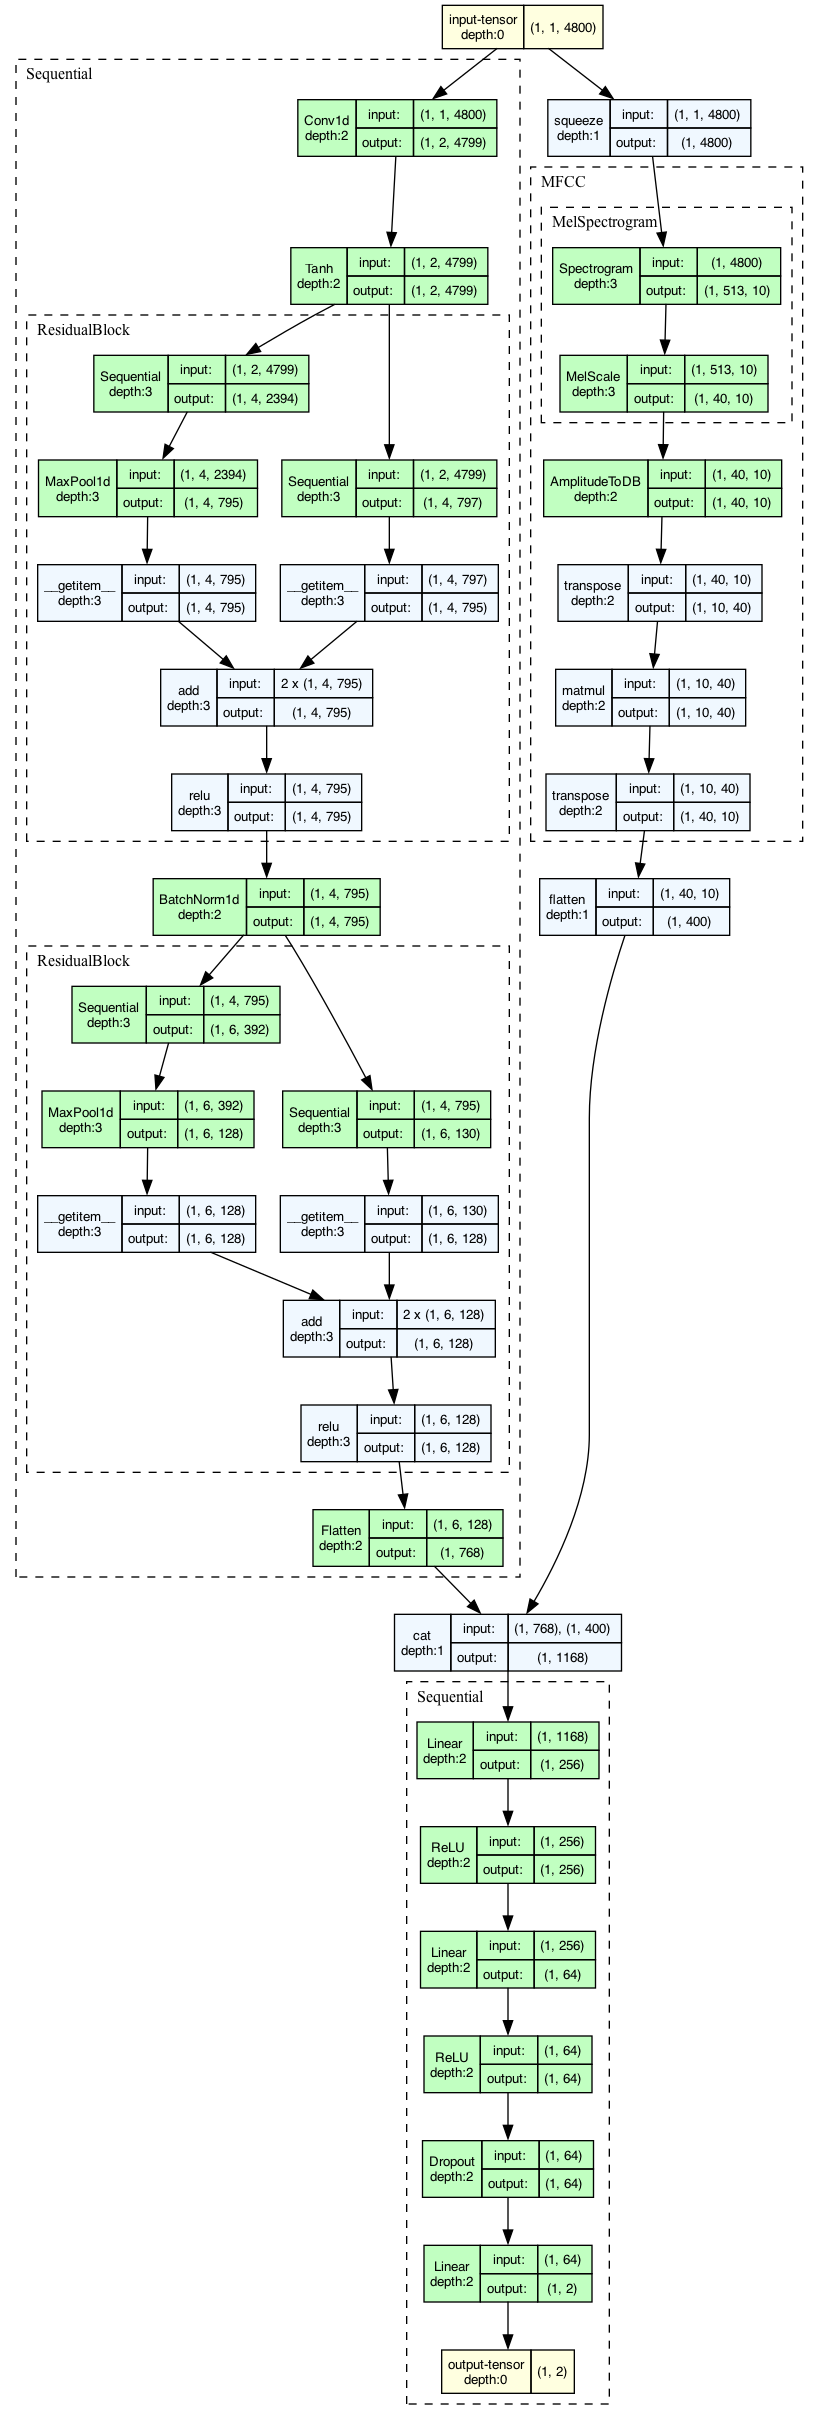
\includegraphics[width=0.15\textwidth]{../assets/final_report_assets/mfcc_resnet_p2_model_arch.png}
  \caption{Phase 2 MFCC + ResNet — Model diagram.}
  \label{fig:phase2_MFCC_resnet_model_architecture}
\end{figure}
\begin{figure}[h]
  \centering
  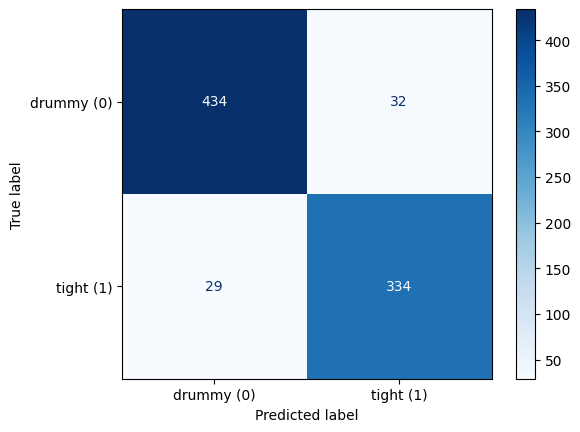
\includegraphics[width=20mm]{../assets/phase2_mfcc_resnet_confusion.png}
  \caption{Phase 2 MFCC + ResNet — Confusion matrix.}
  \label{fig:phase2_mfcc_resnet_confusion}
\end{figure}

\newpage
\section{Model Discussion}
\textbf{Phase 1.} The end-to-end ResNet-style model reached \textbf{98\% accuracy}, outperforming PCA+MLP and SVM baselines.

\textbf{Phase 2.} The \textbf{MFCC + ResNet} model achieved the best overall balance of precision/recall across both classes (0.93 accuracy), closely followed by \textbf{MFCC + MLP} (0.90). Pure waveform ResNet (0.88) also performed strongly.

\medskip
\noindent\textbf{Generalization effects:}
\begin{itemize}
  \item \textbf{Label smoothing} contributed roughly \(\sim\) +2\% accuracy.
  \item \textbf{Tanh} after convolutions added \(\sim\) +2\%, likely by preserving negative polarity in oscillatory signals.
\end{itemize}

\section{Future Work}
\begin{itemize}
  \item Address the discrepancy in input size (Phase 1: 0.75 s / 36k samples; Phase 2: 0.1 s / 4.8k) without resampling—e.g., hierarchical or multi-resolution front ends that accept variable-length inputs.
  \item Design a \textbf{unified architecture} that can process both datasets directly.
  \item Implement a \textbf{robust preprocessing} pipeline to automatically detect \& remove mishits (statistical anomaly detection or similarity search seeded by curated mishits).
\end{itemize}

\section{Conclusion}
Across multiple approaches, \textbf{MFCC + ResNet} delivered the strongest Phase 2 performance with balanced class recall, while an end-to-end \textbf{ResNet} saturated Phase 1 near 98\% accuracy. Small architectural choices (\textbf{label smoothing}, \textbf{tanh}) consistently added measurable gains. Future work will target unified input handling and automated data-quality filtering.
\end{document}